%%% -*-LaTeX-*-

\chapter{Sequence Construction}

With an exact count of viable sequences for level 1, 2, and 3 designs, a mapping from natural numbers to valid trial sequences is now a possibility. Such a mapping would prove valuable for preserving uniformity guarantees, as well as generating solutions more efficiently. This chapter presents an algorithm that guarantees uniformly sampled solutions to level 1, 2, and 3 designs by randomly sampling natural numbers from the uniform distribution in the range of $[0, s)$. Each sampled number is then used to generate the unique trial sequence associated with that number.


\section{Enumerating Permutations and Combinations}

There are several critical components of constructing a solution based on a natural number. In this section, we will review known methods for generating the $n^{th}$ permutation or combination of a set, as well as mapping individual natural numbers to a unique set of numbers that covers the same space using modular arithmetic. All of these techniques will play a major role in solution construction.

\subsection{Interval Mapping}

Suppose we have $n$ numeric intervals, each from $[0, r_n)$. Revisiting the multiplication principle, we can see that there are $m = \prod_1^n r_n$ unique combinations of individual values from each interval. If $j$ is an number selected from $[0, m)$, we can map $j$ to a unique combination of interval value selections using the modulo and division operators. (This technique will still work even when $j \geq m$, but combinations will begin to repeat.)

We begin by computing $j \% r_1$, and saving the result as the selection for the first interval. We then recompute $j$ to be $j = \lfloor \frac{j}{r_1} \rfloor$ before moving on to the next range. This process is repeated for $r_2,r_3,...,r_n$ until the full combination is developed. Figure \ref{fig:interval_breakdown} gives a visual representation of this breakdown for 3 ranges, $r_1 = 3, r_2 = 4$, and $r_3 = 2$.

\begin{figure}
\centering
\centerline{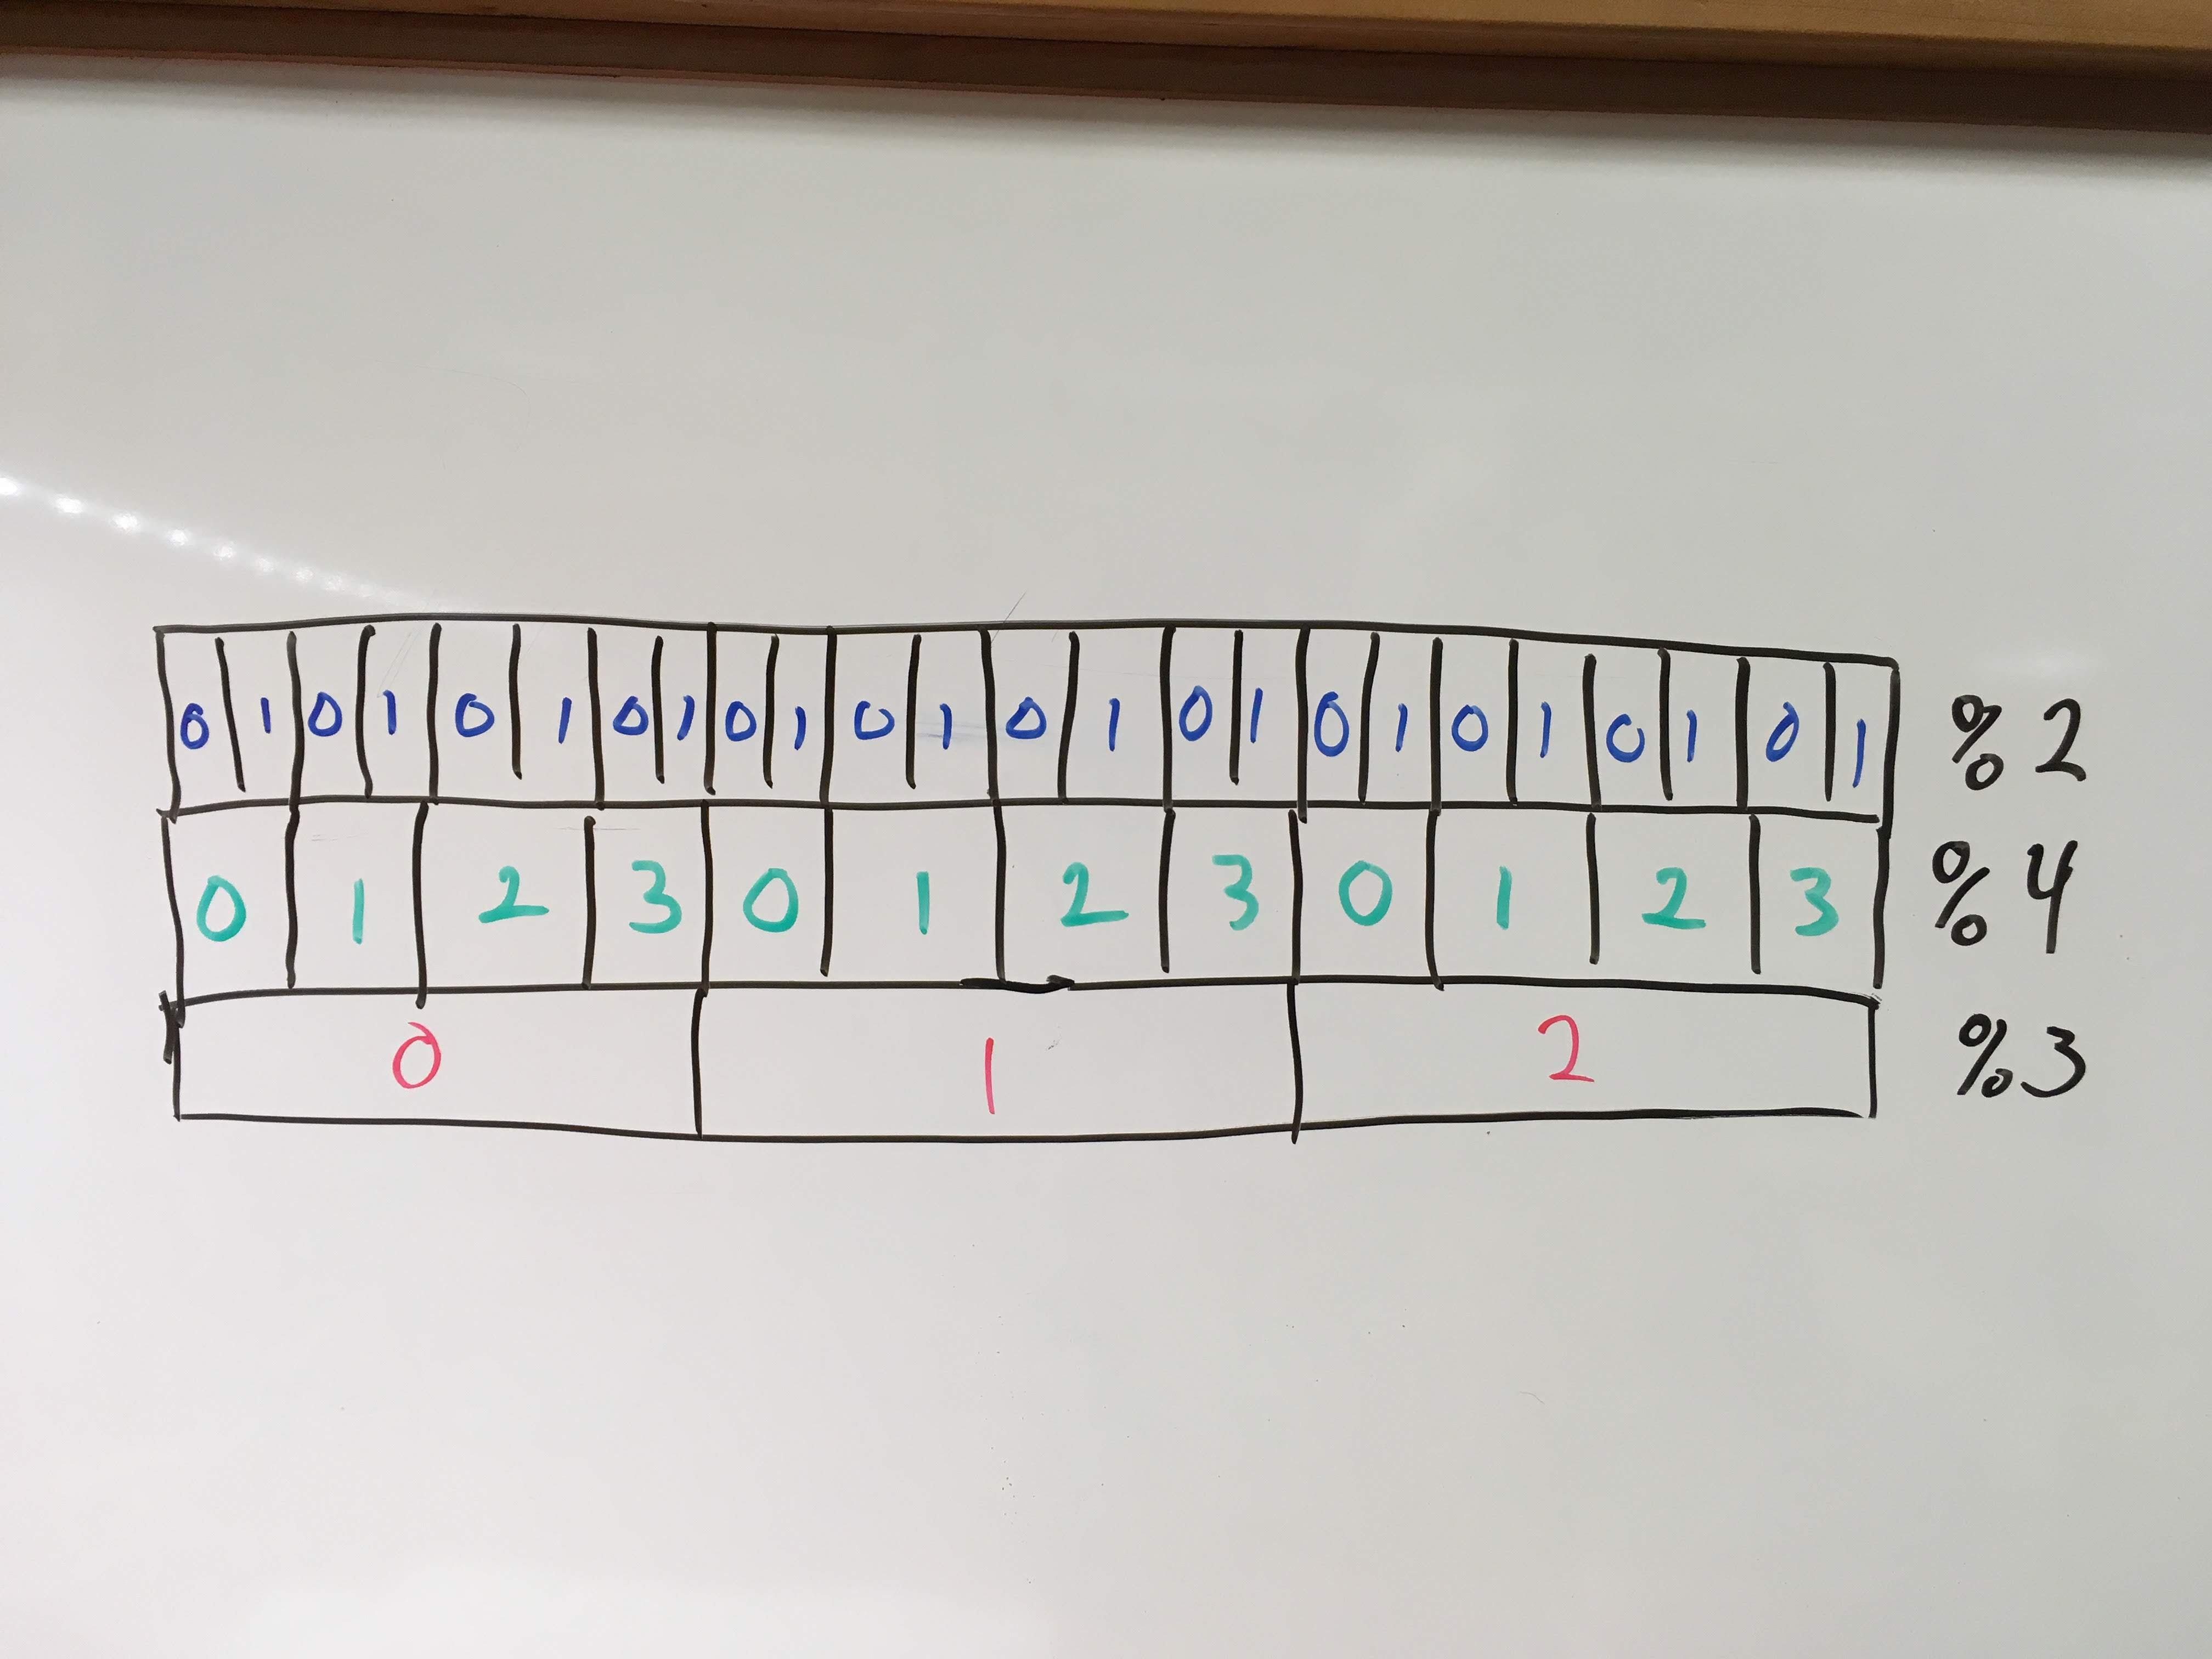
\includegraphics[origin=c,width=12cm]{../figures/interval-breakdown.jpg}}
\caption{Decomposing a Number into Constituent Ranges}
\label{fig:interval_breakdown}
\end{figure}

This technique is used repeatedly in the construction algorithm.

\subsection{Permutations}

Every permutation of a set can be identified by its \textit{inversion} or \textit{inversion sequence}, which loosely-defined, indicates how out-of-order the permutation is when compared with the original sequence. The concept of an inversion was first introduced by Hall \cite{hall_automorphisms_1962}, though we will use on Brualdi's description \cite{brualdi_introductory_2010} here.

Let $S$ be the set of numbers $\{1, 2, ..., n\}$ Suppose we have some permutation $p$ of $S$, $i_1, i_2, ..., i_n$. For each $i$, there exists some finite number of elements in $S$ whose values are greater than $i$, yet precede $i$ in $p$. This is called the inversion for $i$. An inversion sequence, $a_1, a_2, ... a_n$, is the sequence of inversions for a particular permutation of $S$.

For example, because the elements $\{1, 2, 3, 4, 5\}$ are in order, the corresponding inversion sequence for this arrangement is $\{0, 0, 0, 0, 0\}$. If we permute the sequence to obtain $\{2, 5, 4, 1, 3\}$, the associated inversion sequence is $\{3, 0, 2, 1, 0\}$. This can be interpreted to mean that 3 elements larger than 1 precede 1, 0 elements larger than 2 precede 2, 2 elements larger than 3 precede 3, 1 element larger than 4 precedes 4, and 0 elements larger than 5 precede 5. Notice that the final number in an inversion seqeunce must always be 0.

An inversion sequence can be used to generate the associated permutation by using the inversions to select where to place each element. Given an inversion sequence $a_1, a_2, ... a_n$, begin with $n$ empty locations. Beginning with $a_1$, skip $a_i$ empty locations before inserting the $i^{th}$ element of $S$. Using the previous example, this algorithm is demonstrated in Figure \ref{fig:inversion_sequence}.

\begin{figure}
\centering
\centerline{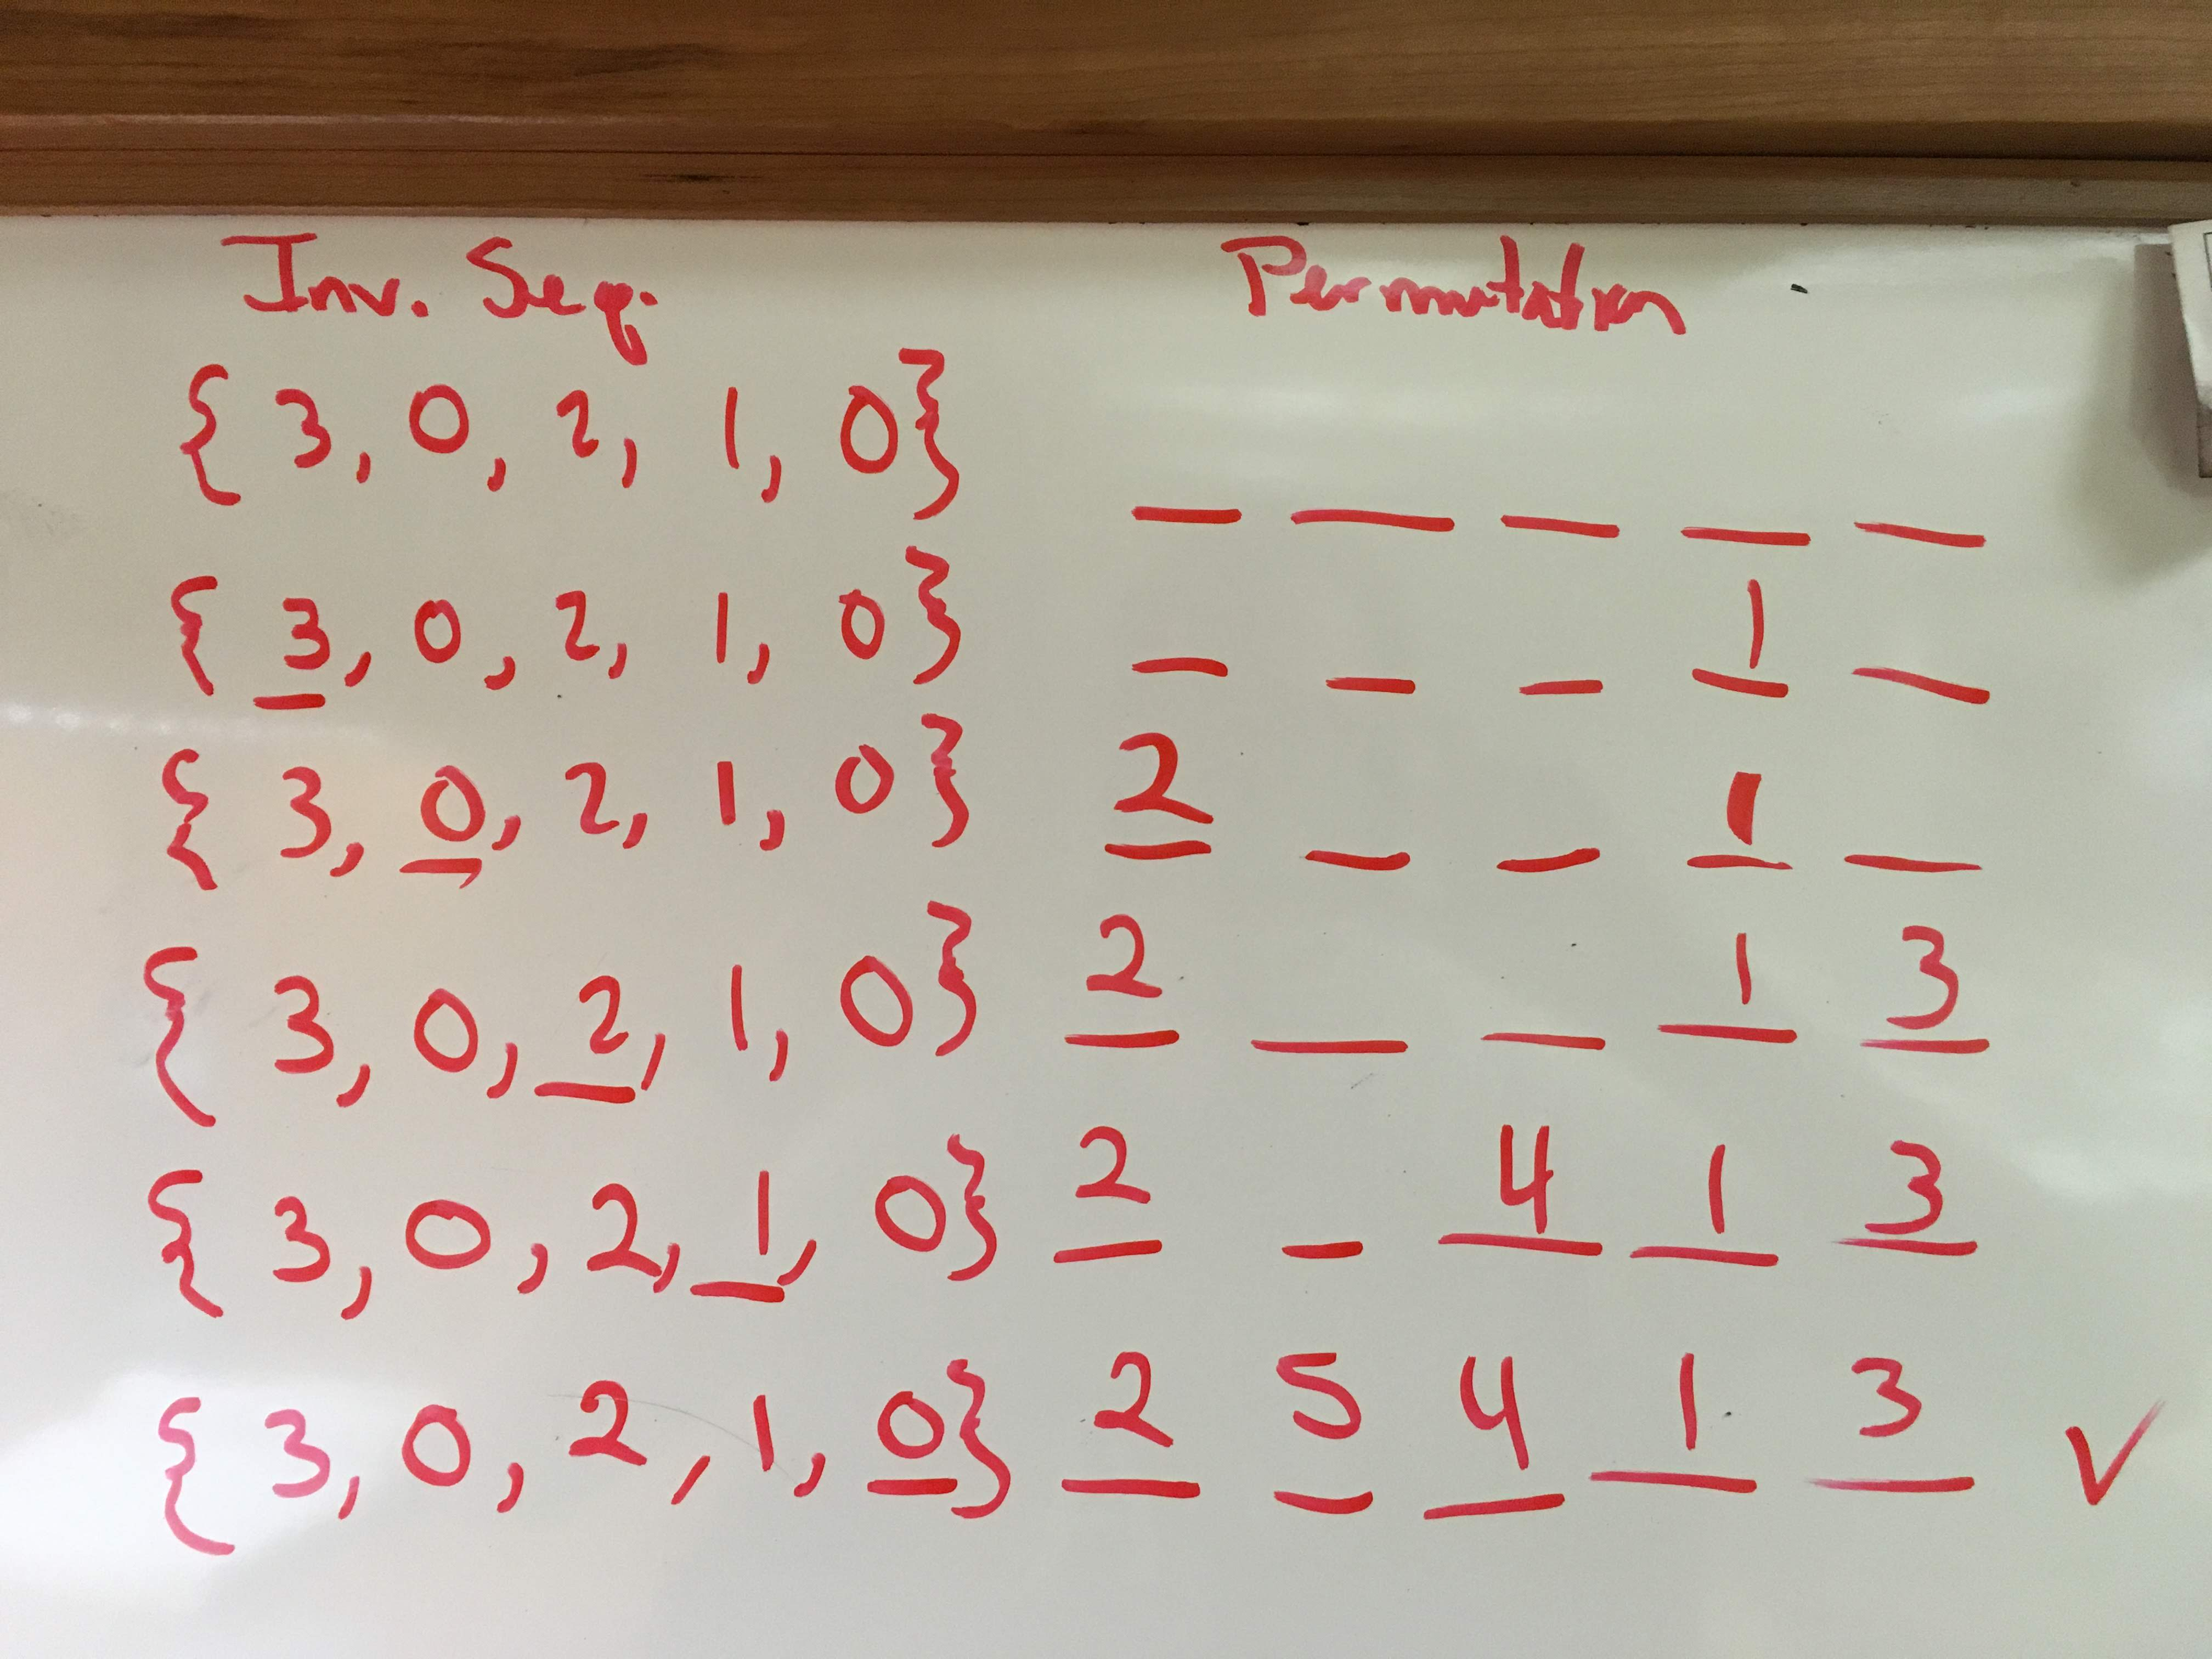
\includegraphics[origin=c,width=12cm]{../figures/inv-seq.jpg}}
\caption{Construction of a Permutation from its Inversion Sequence}
\label{fig:inversion_sequence}
\end{figure}

Finally, we can construct $j^{th}$ inversion sequence of a set by applying the interval mapping technique introduced previously. The maximum value of each position in the inversion sequence is used to construct the intervals. To construct an inversion sequence of $n$ inversions, the limits for the intervals are $\{n, n - 1, n - 2, ..., 2, 1\}$. Lastly a zero is always appended as the final element in the sequence.

\subsection{Combinations}

We can enumerate combinations of a set of elements by again applying the interval mapping technique. For a combination of $r$ elements, taken from a set of $k$ elements, we know that there are $k^r$ possible combinations by the multiplication principle. Applying interval mapping with $r$ intervals, each from $[0, k)$, suffices to enumerate each combination.


\section{Construction Algorithm}

With techniques established for counting solutions and constructing specifc permtutations and combinations, we are now ready to develop the full construction function. At a high level, the construction process has the following steps:

\begin{enumerate}
\item Determine the total number of solutions, $s$, for the design.
\item Randomly sample an integer, $i$, from the uniform distribution in the range $[0, s)$.
\item Use interval mapping to convert $i$ into a unique combination of value selections, $R$, that identify each component of the final solution.
\item Convert each selected value in $R$ to the associated factors and levels. Record them as part of the final solution.
\item Compute the selected values for factors in $\overline{C}_D$ using the previously selected levels for basic factors.
\end{enumerate}

Accomplishing step 1 was the subject of chapter 4. We will not revisit that here. Step 2 relies on the \texttt{randrange} standard library function in Python 3, which produces uniformly-distributed values from an arbitrarily large range. Step 3 is the complicated step, particularly selecting the ranges for interval mapping.

\subsection{Interval Mapping for an Experimental Design}

For level 1, 2, and 3 designs, as we saw in chapter 4, there is a partition of every design containing 5 sets: $\{C_B, C_D, \overline{C}_{B_S}, \overline{C}_{B_I}, \overline{C}_D\}$. In this section we will identify the upper bound of each interval to be used for interval mapping that cover all factors in the partition. We will use $U$ to denote the set of these upper bounds. (The lower bounds are uninteresting, as they are always $0$.

We first consider $C_B$ and $C_D$. Recall that together, these sets contain all factors that are crossed with each other to form the crossing, labeled $X$ in chapter 4. Recall also that $|X|$ governs the length of a generated trial sequence: $l = |X|$, and that there are $l!$ permtutations of the ordered pairs in $X$. Therefore, the first interval, which will determine which permutation of $X$ to use, is $l!$. At this point, $U = \{l!\}$.

The next set in the partition is $\overline{C}_{B_S}$, which is the set of basic factors that are \textit{not} included in $C_B$, but are sources of data for factors in $C_D$, and are therefore governed by the values associated with the chosen permutation for a given solution. Recall from chapter 4 that we defined $X_S$ to represent the source crossing, and that there is a distinct subset of $X_S$, $J_n$, that represents the source crossings that are compatible with the $n^{th}$ ordered pair in $X$. We also defined $S$ to be the set of these subsets. We need a distinct interval for each of these subsets, so we add $l$ values to $U$, one for the size of each subset in $S$. $U$ will now contain $l + 1$ elements: $U = \{l!, |J_1|, |J_2|, ..., |J_l|\}$.

Lastly, we consider $\overline{C}_{B_I}$. ($\overline{C}_D$ also remains in the partition, but values for factors in this set are governed by other basic factors, and will be determined in step 5. No additional intervals need be computed.) Recall that $\overline{C}_{B_I}$ represents the set of basic factors that are completely independent, meaning they are not governed by any factors in $C_D$. Because they are completely independent, every possible $l$-combination of levels for each factor in $\overline{C}_{B_I}$ is valid. Therefore an interval must also be added for each factor $f$ with upper bound $|f|^l$. (Recall that $|f|$ denotes the number of levels of factor $f$.) $U$ is now complete:

\[
U = \{ l!, |J_1|, |J_2|, ..., |J_l|, |f_1|^l, |f_2|^l, ..., |f_i|^l\}
\]

Where $f_i$ represents the $i^{th}$ factor in $\overline{C}_{B_I}$. Interestingly, the upper bounds in $U$ are the same values which were multiplied together in chapter 4 to produce the total solution count.

\subsection{Mapping Selected Values to Levels}

Once a value has been produced for each interval, the next step is to produce the correct levels or level sequences for each factor associated with that interval. The selected permutation value is converted to a unique inversion sequence using interval mapping, which sequence is then used to construct the permutation. This permutation of integers is then converted into a seqeuence of level values by using each integer as an index into the ordered pairs in $X$.

The selected values for independent basic factors are converted in similar fashion. Each selected value identifies a combination number, which is converted to a set of values using interval mapping. Each value is an index into the list of levels for the associated factor.

Lastly, the selected values for source combinations must be converted. These are slightly more complex, as the viable combinations vary based on the selected levels for each trial. It would be incorrect to select a source combination from the $n^{th}$ set of valid source combinations for the $n^{th}$ trial, because the permutation may have shifted the position of the original $n^{th}$ trial in the sequence. A mult-level indexing scheme is employed to ensure that the selected value is used to map exclusively to valid combinations, in which the permtuted values are used to index into the correct set of valid source combinations. This is shown in Figure \ref{fig:source_combinations}.

\begin{figure}
\centering
\centerline{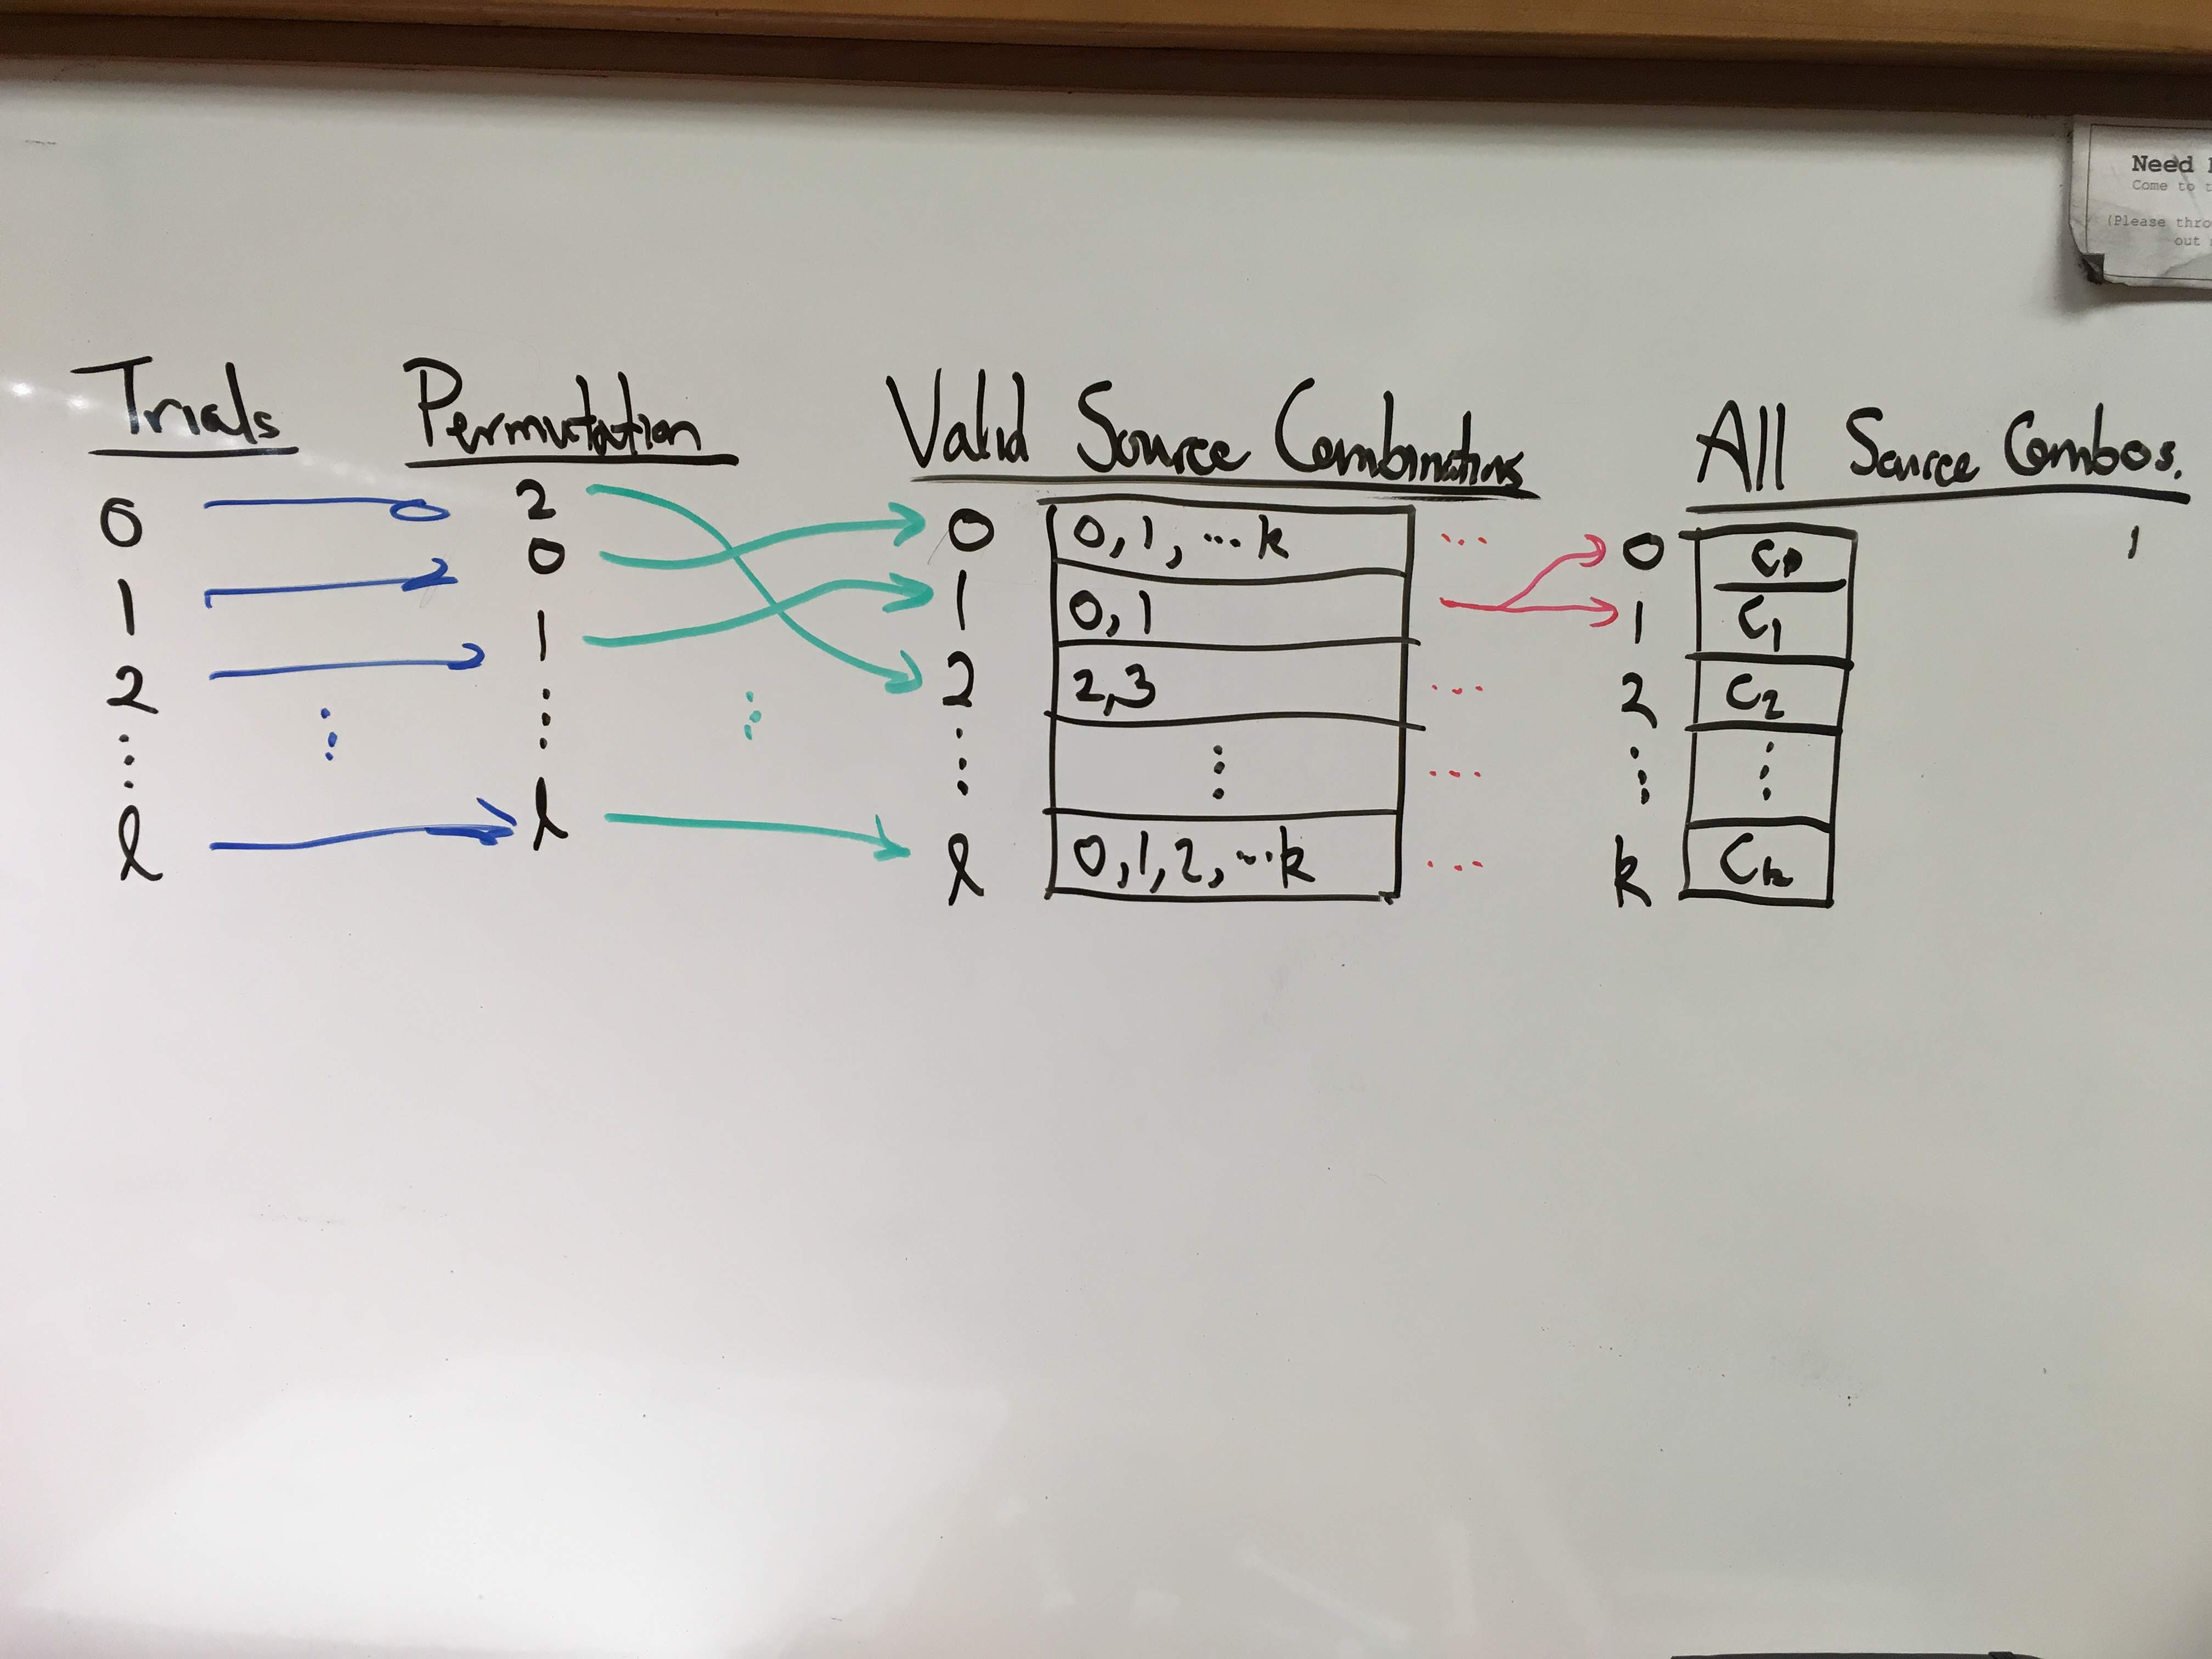
\includegraphics[origin=c,width=12cm]{../figures/source-combinations.jpg}}
\caption{Selecting Valid Source Combinations}
\label{fig:source_combinations}
\end{figure}

For example, if the selected permutation places the original crossing value for trial number 2 in the zeroth position in the sequence (trial 0), then the source combination for trial 0 must also be selected from the valid source combinations originally generated for trial number 2.


\section{Example}

TODO

\section{Handling Constraints}

Recall that the complexity gradation did not account for the external constraints that may be applied to a design. Such constraints typically enforce some kind of rule regarding repetition of particular characteristics. For example, in the design for Stroop experiments, it is common to apply a constraint that requires that the generated sequence never contain two or more congruent trials in sequence. Constraints may be applied to the levels of derived factors as well, therefore the use may impose practically any condition upon the generated sequence.

In the future, the counting and construction algorithms could be enhanced to account for these constraints. This will be discussed further in Chapter 7. In the meantime however, basic rejection sampling is applied ensure that no generated sequences that violate constraints are ever returned to the user. All constraints are represented in the original SAT encoding, which allows us to invoke a SAT sampler with added clauses representing the constructed sequence to verify that the constructed sequence is in fact valid. More details will be provided in the benchmarks section.


\section{Benchmarks}

% TODO: Repeat benchmarks from chapter 2 that apply here.

Of the ten benchmarks designs that were introduced in chapter 2, 4 can be classified as level 1, 2, or 3 designs: \texttt{stroop-2}, \texttt{stroop-3}, \texttt{stroop-4}, \texttt{stroop-5}. We will repeat the benchmarks for those designs here using this construction approach to sampling. We will also introduce a few additional designs involving variations on the Stroop design to demonstrate the scalability of this approach, and the empirical performance of the rejection sampling phase. Table \ref{tab:benchmark_experiments} reviews the basic experiment data for each benchmark design. Table \ref{tab:sampling_metrics} summarizes the time required to generate 10,000 samples for each design, as well as the average number of rejections per sample. (Rejctions caused by constructing a trial sequence that violated external constraints.)

\begin{table}
  \centering
  \caption{Benchmark Experiments}
\begin{tabular}{|c|c|c|c|c|}
\hline
\multicolumn{1}{|l|}{Experiment Name} & Sequence Length & Total Solutions & Generate Single Solution  \\ \hline
stroop-2                              & 4               & 12              &                           \\ \hline
stroop-3                              & 9               & 151,200         &                           \\ \hline
stroop-4                              & 16              &                 &                           \\ \hline
stroop-5                              & 25              &                 &                           \\ \hline
stroop-10                             &                 &                 &                           \\ \hline
stroop-20                             &                 &                 &                           \\ \hline
stroop-20-constraints                 &                 &                 &                           \\ \hline
\end{tabular}
\label{tab:benchmark_experiments}
\end{table}

\begin{table}
  \centering
  \caption{Sampling Metrics}
\begin{tabular}{|c|c|c|c|c|}
\hline
\multicolumn{1}{|l|}{Experiment Name} & 10,000 Samples & Avg. Rejections/Sample  \\ \hline
stroop-2                              &                &                         \\ \hline
stroop-3                              &                &                         \\ \hline
stroop-4                              &                &                         \\ \hline
stroop-5                              &                &                         \\ \hline
stroop-10                             &                &                         \\ \hline
stroop-20                             &                &                         \\ \hline
stroop-20-constraints                 &                &                         \\ \hline
\end{tabular}
\label{tab:sampling_metrics}
\end{table}

